% $Id: template.tex 11 2007-04-03 22:25:53Z jpeltier $

\documentclass{vgtc}                          % final (conference style)
%\documentclass[review]{vgtc}                 % review
%\documentclass[widereview]{vgtc}             % wide-spaced review
%\documentclass[preprint]{vgtc}               % preprint
%\documentclass[electronic]{vgtc}             % electronic version

%% Uncomment one of the lines above depending on where your paper is
%% in the conference process. ``review'' and ``widereview'' are for review
%% submission, ``preprint'' is for pre-publication, and the final version
%% doesn't use a specific qualifier. Further, ``electronic'' includes
%% hyperreferences for more convenient online viewing.

%% Please use one of the ``review'' options in combination with the
%% assigned online id (see below) ONLY if your paper uses a double blind
%% review process. Some conferences, like IEEE Vis and InfoVis, have NOT
%% in the past.

%% Figures should be in CMYK or Grey scale format, otherwise, colour
%% shifting may occur during the printing process.

%% These few lines make a distinction between latex and pdflatex calls and they
%% bring in essential packages for graphics and font handling.
%% Note that due to the \DeclareGraphicsExtensions{} call it is no longer necessary
%% to provide the the path and extension of a graphics file:
%% \includegraphics{diamondrule} is completely sufficient.
%%
\ifpdf%                                % if we use pdflatex
  \pdfoutput=1\relax                   % create PDFs from pdfLaTeX
  \pdfcompresslevel=9                  % PDF Compression
  \pdfoptionpdfminorversion=7          % create PDF 1.7
  \ExecuteOptions{pdftex}
  \usepackage{graphicx}                % allow us to embed graphics files
  \DeclareGraphicsExtensions{.pdf,.png,.jpg,.jpeg} % for pdflatex we expect .pdf, .png, or .jpg files
\else%                                 % else we use pure latex
  \ExecuteOptions{dvips}
  \usepackage{graphicx}                % allow us to embed graphics files
  \DeclareGraphicsExtensions{.eps}     % for pure latex we expect eps files
\fi%

%% it is recomended to use ``\autoref{sec:bla}'' instead of ``Fig.~\ref{sec:bla}''
\graphicspath{{figures/}{pictures/}{images/}{./}} % where to search for the images

\usepackage{microtype}                 % use micro-typography (slightly more compact, better to read)
\PassOptionsToPackage{warn}{textcomp}  % to address font issues with \textrightarrow
\usepackage{textcomp}                  % use better special symbols
\usepackage{mathptmx}                  % use matching math font
\usepackage{times}                     % we use Times as the main font
\renewcommand*\ttdefault{txtt}         % a nicer typewriter font
\usepackage{cite}                      % needed to automatically sort the references
\usepackage{subcaption}
\usepackage{algorithm}
\usepackage{algpseudocode}
\usepackage{url}
\usepackage{placeins}
%% We encourage the use of mathptmx for consistent usage of times font
%% throughout the proceedings. However, if you encounter conflicts
%% with other math-related packages, you may want to disable it.


%% If you are submitting a paper to a conference for review with a double
%% blind reviewing process, please replace the value ``0'' below with your
%% OnlineID. Otherwise, you may safely leave it at ``0''.
\onlineid{0}

%% declare the category of your paper, only shown in review mode
\vgtccategory{Research}

%% allow for this line if you want the electronic option to work properly
%% \vgtcinsertpkg

%% In preprint mode you may define your own headline.
%\preprinttext{To appear in an IEEE VGTC sponsored conference.}

%% Paper title.

\title{OPTICSvis: Visualizing the OPTICS algorithm}

%% This is how authors are specified in the conference style

%% Author and Affiliation (single author).
%%\author{Roy G. Biv\thanks{e-mail: roy.g.biv@aol.com}}
%%\affiliation{\scriptsize Allied Widgets Research}

%% Author and Affiliation (multiple authors with single affiliations).
%%\author{Roy G. Biv\thanks{e-mail: roy.g.biv@aol.com} %
%%\and Ed Grimley\thanks{e-mail:ed.grimley@aol.com} %
%%\and Martha Stewart\thanks{e-mail:martha.stewart@marthastewart.com}}
%%\affiliation{\scriptsize Martha Stewart Enterprises \\ Microsoft Research}

%% Author and Affiliation (multiple authors with multiple affiliations)
\author{Sonja Biedermann\thanks{e-mail:sonja.biedermann@univie.ac.at }\\ %
        \scriptsize University of Vienna %
\and Christian Permann\thanks{e-mail:a01463926@unet.univie.ac.at}\\ %
     \scriptsize  University of Vienna}

%% A teaser figure can be included as follows, but is not recommended since
%% the space is now taken up by a full width abstract.
%\teaser{
%  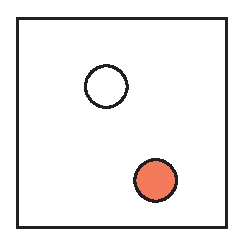
\includegraphics[width=1.5in]{sample.eps}
%  \caption{Lookit! Lookit!}
%}

%% Abstract section.
\abstract{Duis autem vel eum iriure dolor in hendrerit in vulputate
velit esse molestie consequat, vel illum dolore eu feugiat nulla
facilisis at vero eros et accumsan et iusto odio dignissim qui blandit
praesent luptatum zzril delenit augue duis dolore te feugait nulla
facilisi. Lorem ipsum dolor sit amet, consectetuer adipiscing elit,
sed diam nonummy nibh euismod tincidunt ut laoreet dolore magna
aliquam erat volutpat. Ut wisi enim ad minim veniam, quis nostrud exerci tation ullamcorper
suscipit lobortis nisl ut aliquip ex ea commodo consequat. Duis autem
vel eum iriure dolor in hendrerit in vulputate velit esse molestie
consequat, vel illum dolore eu feugiat nulla facilisis at vero eros et
accumsan et iusto odio dignissim qui blandit praesent luptatum zzril
delenit augue duis dolore te feugait nulla facilisi.%
} % end of abstract

%% ACM Computing Classification System (CCS).
%% See <http://www.acm.org/about/class> for details.
%% We recommend the 2012 system <http://www.acm.org/about/class/class/2012>
%% For the 2012 system use the ``\CCScatTwelve'' which command takes four arguments.
%% The 1998 system <http://www.acm.org/about/class/class/2012> is still possible
%% For the 1998 system use the ``\CCScat'' which command takes four arguments.
%% In both cases the last two arguments (1998) or last three (2012) can be empty.

\CCScatlist{
  \CCScatTwelve{Human-centered computing}{Visu\-al\-iza\-tion}{Visu\-al\-iza\-tion techniques}{Treemaps};
  \CCScatTwelve{Human-centered computing}{Visu\-al\-iza\-tion}{Visualization design and evaluation methods}{}
}

%\CCScatlist{
  %\CCScat{H.5.2}{User Interfaces}{User Interfaces}{Graphical user interfaces (GUI)}{};
  %\CCScat{H.5.m}{Information Interfaces and Presentation}{Miscellaneous}{}{}
%}

%% Copyright space is enabled by default as required by guidelines.
%% It is disabled by the 'review' option or via the following command:
% \nocopyrightspace

%%%%%%%%%%%%%%%%%%%%%%%%%%%%%%%%%%%%%%%%%%%%%%%%%%%%%%%%%%%%%%%%
%%%%%%%%%%%%%%%%%%%%%% START OF THE PAPER %%%%%%%%%%%%%%%%%%%%%%
%%%%%%%%%%%%%%%%%%%%%%%%%%%%%%%%%%%%%%%%%%%%%%%%%%%%%%%%%%%%%%%%%

\begin{document}
%% The ``\maketitle'' command must be the first command after the
%% ``\begin{document}'' command. It prepares and prints the title block.

%% the only exception to this rule is the \firstsection command
\firstsection{Introduction} % sonja

\maketitle

%% \section{Introduction} %for journal use above \firstsection{..} instead

OPTICS is a popular and robust density-based clustering algorithm for spatial
data. Although popular, the output generated by OPTICS has a tendency to appear
somewhat cryptical---instead of generating a straightforward mapping of points
to cluster-IDs, it outputs a list of points adjoined with metadata. This output
format holds not one, but many clusterings which still need to be extracted.

This is done by picking a \emph{cutoff}, which then separates all points that
fall below this value into a cluster. As this is not easy to conceptualize, the
output of the algorithm is usually visualized using a bar chart---as such, it
can be argued that visualization is already are core part of working with
OPTICS, and leads us to our motivation to implement a more sophisticated and
interactive visualization design.

\section{Motivation} %% sonja

OPTICS is often taught to undergrad students among a group of other clustering
algorithms such as k-Means and DBSCAN. A distinguishing feature of OPTICS among
this group is that the output is not yet a clustering, but rather an
intermediary output that still needs some parameterization---called the
\emph{cutoff}---before yielding a clustering that can be used by e.g. producing
a colored scatterplot of the input data.

This parameterization is oftentimes puzzling to students. How is this value
picked? The real-world answer to this is often to just try out a few values and
observe the resulting clustering. Although some gut feeling as to picking this
value develops in routine users of this algorithm, it is still hard to pass
onto students.

We want to offer a visualization dashboard that allows students to
interactively try out the algorithm on data sets of their choice. Both the
cutoff and the two other important parameters, $\varepsilon$ and \emph{minPts}, can
be set and their effect observed. Lastly, we also introduce a dendrogram view
that is relatively uncommon when dealing with OPTICS, as it is not an hierachial
algorithm per se, but still capable of producing hierarchies of clusterings
that might be worthwhile to study. The hierarchies are a direct result of
choosing different cutoff values and thus also serve to motivate the meaning of
differing cutoff values.

\subsection{Background information}

What follows are a few facts that are either needed to understand the rest
of the paper or are distinguishing general characteristics of the project,
such as tasks or user target groups.

\subsubsection{OPTICS}

As already discussed, OPTICS is a density-based clustering algorithm that works
on spatial data. Density-based clustering algorithms typically classify points
into either cluster points (possibly giving them a cluster ID) or noise, which
is made up of points that belong to regions that are not dense enough to be
considered clusters.

More concretely, OPTICS computes its output representation by jumping between
points (the choice of the first point is left in the open) and performing
$\varepsilon$-neighborhood queries. The $\varepsilon$ parameter supplied to the
algorithm is used. Note that $\varepsilon$ may very well be set to an
outrageously high value, but will then result in an algorithmic complexity of
$O(n^2)$ as every neighborhood query would likely return the entire data set.

The influence of the \emph{minPts} parameter on the result is twofold: first,
the \emph{core distance} of a point is defined as the distance to its
\emph{minPts}th neighbor. Secondly, a point that fails to have \emph{minPts}
neighbors is considered to be unreachable by the algorithm and will thus
certainly be labeled as noise later on.


\subsubsection{Data}

Our visualization dashboard is capable of dealing with scalar, two dimensional
data. We provide both predefined data sets that showcase the very robust
behavior of OPTICS, e.g. by having data sets that form circles or spirals,
objects that would not be correctly classified by the likes of k-Means and
DBSCAN, and a text input field that allows the user to input her own data.

Although higher dimensional data is not supported, more dimensions can be
supplied and then two dimensions chosen. The other dimensions are not
considered. Albeit being limited, this still allows to explore a higher
dimensional data set in slices, and dimensionality reduction can be done
using external tools if so desired.


\subsubsection{Users}

Our visualization design has a strong focus on education. As such, our targeted
user groups are educational staff, such as lecturers, students (mainly
undergrad level), but also researchers that have a more casual need for using
OPTICS or may be casually evaluating the algorithm for further use. Our
application is not designed to work well with larger data sets, which we
consider non-casual use, although non-interactive elements are still
functional---interactive elements, however, often rely on hovering over bars or
points, which will become unusable if there are many bars or points. These
aspects are, however, geared towards the educational experience that a student
may have; and students are unlikely to want to figure out how an algorithm
works by loading up a large data set. It is also of note that the realized
product is a browser application and is thus severely limited in terms of
computational power.


\subsubsection{Tasks}

The main task our implementation aims to help with, is to educate on how use OPTICS and to see if it fits given data and problem.

Teachers can either use our default data set or load a custom data set to explain how the algorithm works. They could use our implementation as a means of presentation and to show how parameter changes affect the output. The different views are also supposed to help understanding what the output actually means. Beeing able to play arround with parameters and having different usefull views could be beneficial for understanding the algorithm itself.

The second use-case in our mind was for researchers or anyone interested to find out if they want to do future work with this algorithm. For this they will probably just play around with our implementation to see if they want to put further work into OPTICS. Researchers may additionaly want to test their data set or part of it with our tool.



\section{Related work} %% sonja

\subsection{Other visualization solutions}
 Not many tools exist that take on this subject, although notable projects exist, especially Clustervision\cite{Clustervision} and a DBSCAN visualization that we found \cite{DBSCAN}, the latter of which only visualizes how DBSCAN goes about finding clusters (i.e. shows the epsilon neighborhoods). It is notable that DBSCAN results in a simple partition of points into clusters along with some metadata (e.g. core points versus edge points).
\subsection{Previous visualization ideas}
(-that you incorporated into your solution)
Mockups on Website(some text also reusable?)
\subsection{References}
(- to both academic and commercial tools used)
Maybe we don't need this section, since we talk about this elsewhere (e.g. implementation)



\section{Approach} %% sonja

We split our work on the visualization design into two parts: first, we
designed and implemented the static views, making sure that even without
interactivity, they display useful information---providing an overview. Only
afterward we added filtering, brushing and zooming to get at some details that
are hidden in the overview or provide value during presentations in an
educational setting (e.g. a classroom).

\subsection{Views}

Our visualization design encompasses 6 views showing either the input data or
different aspects of the output data. Perhaps most central is the reachability
chart, which is the staple bar chart that was proposed as the go-to
visualization method by the authors of OPTICS~\cite{optics}. We have extended
this view to contain an interactive bar that corresponds to the cutoff value.
Changes to this bar result in a recalculation of the output clustering. We have
also introduced a second cutoff to separate subclusters from their
superclusters (e.g. even denser regions in an already dense region).

The top left view shows a density map of the input data. This serves as a reminder
of what the OPTICS algorithm deals with---densities---and shows the general shapes of
the data. The density map is estimated using a Gaussian kernel and will thus show
circular tendencies that may not fit the data perfectly.

The actual data points on this view are hidden, but can be toggled by double clicking
the canvas. Doing this will show the cluster IDs of the points mapped to a color, and
also allow the selection of points using a lasso. The corresponding bars of the reachability
chart will then be highlighted. This is a means to substantiate how each bar of the
reachability correlates to a point in the data set to be used during e.g. in-class
discussion of the algorithm.

Going clockwise from this view, the next view shows a bar chart that summarizes the
clustering by the cluster sizes. Very unbalanced values may be indicative of a bad
configuration.

The next view visualizes the path that the algorithm took during execution.
Hovering a bar of the reachability chart will highlight (by increasing the
stroke width) the corresponding path. This is useful for tracing the algorithm
on small data sets (e.g. when doing homework on the algorithm) and shows the
decisions that the algorithm made during a run. Changes to the paths taken when
changing the configuration do not seem significant as to the quality of the
configuration.

The heatmap that is next is a rather novel way to help the user find the most
natural clustering of the given data set as well as show hierarchial clusters.
For this visualization, we apply the data set to both axes in the order that is
given by the OPTICS algorithm. For each pair $(p_i, p_j) \in DB \times
DB$, where $DB$ is the data set or data base, we compute the distance
$d(p_i, p_j)$ and map it to a hue, with darker hues bound to smaller distances.
Note that this is the actual distance between points (given by e.g. the
Euclidian distance function), and not the core dist as defined previously.

If the data set has a clustering structure that is apparent with the given
configuration of $\varepsilon$ and \emph{minPts}, the clusters will become
apparent as squares of darker color. Figure~\ref{fig:heatmap} shows this for a
small data set. Other characteristics are also visible---such as having
circular objects in the data set, which will appear as diagonal lines in the
heatmap. Although this information is also visible in the reachability
plot---where clusters appear as valleys---we have experienced that the squares
are easier to grasp for novices, and squares seem to be easier to perceive
especially with subcluster structures, which will appear as nested groups of
squares. This view supports a square brush which can be used to select regions
of the data set and will highlight the corresponding data points in the
reachability chart.

A particularly bad choice of parameterization will also become apparent in the
heatmap, as it will appear rather erratic, as shown in
Figure~\ref{fig:heatmap-bad}.

\begin{figure}[tb]
    \centering

    \begin{subfigure}{0.45\columnwidth}
        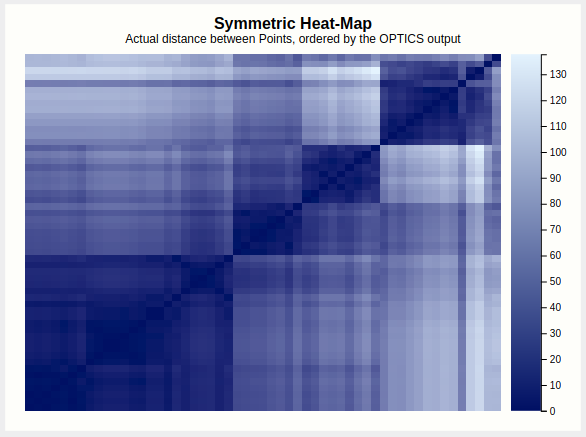
\includegraphics[width=\columnwidth]{heatmap}
        \caption{}
        \label{fig:heatmap}
    \end{subfigure}%
    \hspace{1em}
    \begin{subfigure}{0.45\columnwidth}
        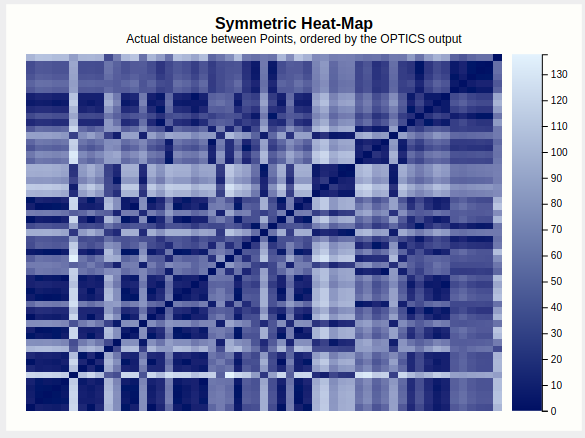
\includegraphics[width=\columnwidth]{heatmap-bad}
        \caption{}
        \label{fig:heatmap-bad}
    \end{subfigure}
    \caption{Heatmap. (a) A good configuration. (b) A bad one.}
\end{figure}

The final view is hidden initially. By double clicking the reachability plot, a
large dendrogram view will appear. Due to constraints in visualization estate,
this dendrogram is flipped on its size and is also not technically a dendrogram---but
rather a general tree, as leaves are not forcefully pulled to the last level.

A dendrogram is without doubt a good choice when visualizing hierarchies, which
is our aim. However, it should also be noted that for large data sets, a
dendrogram does not scale, and analyzing large hierarchies will quickly turn
into an ordeal.  Possible mitigations include e.g. collapsing parts of the tree
or zooms, but the original problem still remains. Such was also argued
in~\cite{optics}, where the authors make a point of highlighting that the
typical reachability chart is vastly superior to tree-like outputs of
other---usually hierarchical---algorithms. We want to point out that OPTICS is
\emph{not} a hierarchical algorithm, but merely \emph{also} mirrors the
hierarchical structures of the input in its output. Hierarchical clustering
algorithms typically work by recursively merging (bottom-up) or splitting
(top-down) a trivial clustering.  OPTICS does not show this behavior.

The question is: how to source the hierarchy given the output, if it is not
just given by how the algorithm does its clustering? We have chosen a rather
simplistic approach, consisting of descendingly sorting the algorithm output by
the core distance of each point, and then for every distance, extracting the
clustering that results when setting the cutoff to this distance. If this
clustering contains at least one cluster ID that is not present in the last
clustering (if any), then some cluster must have split---and the current
clustering is the next hierarchy level.  We completely ignore points that get
assigned noise status.  However, since points drop out of the clustering, we
may overlook clusterings that are significantly different, but have as many as
or less clusters than the previous. Thus, the resulting hierarchy is only
approximate, but a few radically different clusterings (``cornerstone
clusterings'') are guaranteed to be contained, and each lower hierarchy level
is larger than the last, something that is always given when working with
hierarchial clustering algorithms.

Any level of the hierarchy can be selected, which results in the application of
the corresponding cutoff to the main visualization (as if having dragged the
cutoff bar to this position). This way, certain levels of the hierachy can be
nicely mapped to the reachability chart, which also serves to illustrate how
hierarchies appear in this more canonical chart type.

\subsection{Interactivity}

\subsection{Discussion}



\section{Implementation} %% sonja

The dashboard is implemented using JavaScript and the fantastic d3.js SVG and DOM
manipulation library. The application is entirely client-side and only needs a
file server to run. A current version is also available
online\footnote{\url{https://biederfrau.github.io/opticsvis/app/index.html}}.

The project also contains a complete implementation of OPTICS which is slightly tweaked to
generate information used in some charts (e.g. the jump paths). This has the downside
that our implementation might be a bit slower, although in general, the bottleneck seems
to be the SVG rendering in the browser.

The application was tested on somewhat recent versions of Google Chrome and Mozilla Firefox
and found to be in good working order in both. However, we noted that Firefox performs noticeably
worse with regard to SVG rendering, so much so that it actively struggles loading
some data sets. This seems more pronounced on Windows, whereas on Linux the issue is less pronounced
(although still significantly worse than Chrome). We thus dearly recommend using it in
Chrome and hope that Firefox will get its rendering act together sometime soon.

\subsection{Challenges}
\begin{itemize}
\item The OPTICS implementation isn't the most efficient one and it may be a good idea to have a backend for the calculations.
\item We found it difficult to force the brush on top of the heat-map in a position where it makes sense, because since the x and y-Axis are mirrored, any non square selection doesn't make sense.
\item We think the main problem that remains is how to make it behave well with larger inputs. Given a bad configuration (mainly a very large  $\varepsilon$), OPTICS runs in quadratic time, and some components such as our scented widget will call the algorithm every time an input event is triggered, which may lead to an explosion of calls which all take $ n^{2} $ time. This can't really be avoided (the output is needed to render the scented part), but maybe caching would cushion this effect. However, this depends on how often the same configurations would reappear, which may not be all that often.
\item There seem to be performance issues with Firefox and large data sets, which we were not able to solve yet.
\end{itemize}


\section{Results}

We feel, that our implementation\cite{Our_Implementation} is most usefull when used to explain OPTICS and learning to understand its output. It is best used with at least a small amount of knowledge about density based clustering or in combination with learning about it. This is possibly the only tool that allows for interactive visual experimentation with this algorithm.

\subsection{Scenarios of use}

A scenario in which a teacher at a university may use our implementation may look something like the following:

First the teacher could show the default view, that appears when loading the tool, to his students. Here a good parameter set is preselected and we can clearly see the clusterstructure on the data. The actual problem of clustering can be presented here as well as the specifics about density based clustering in comparison the methods like k-Means, that have probably been discussed in an earlier lecture.

\noindent
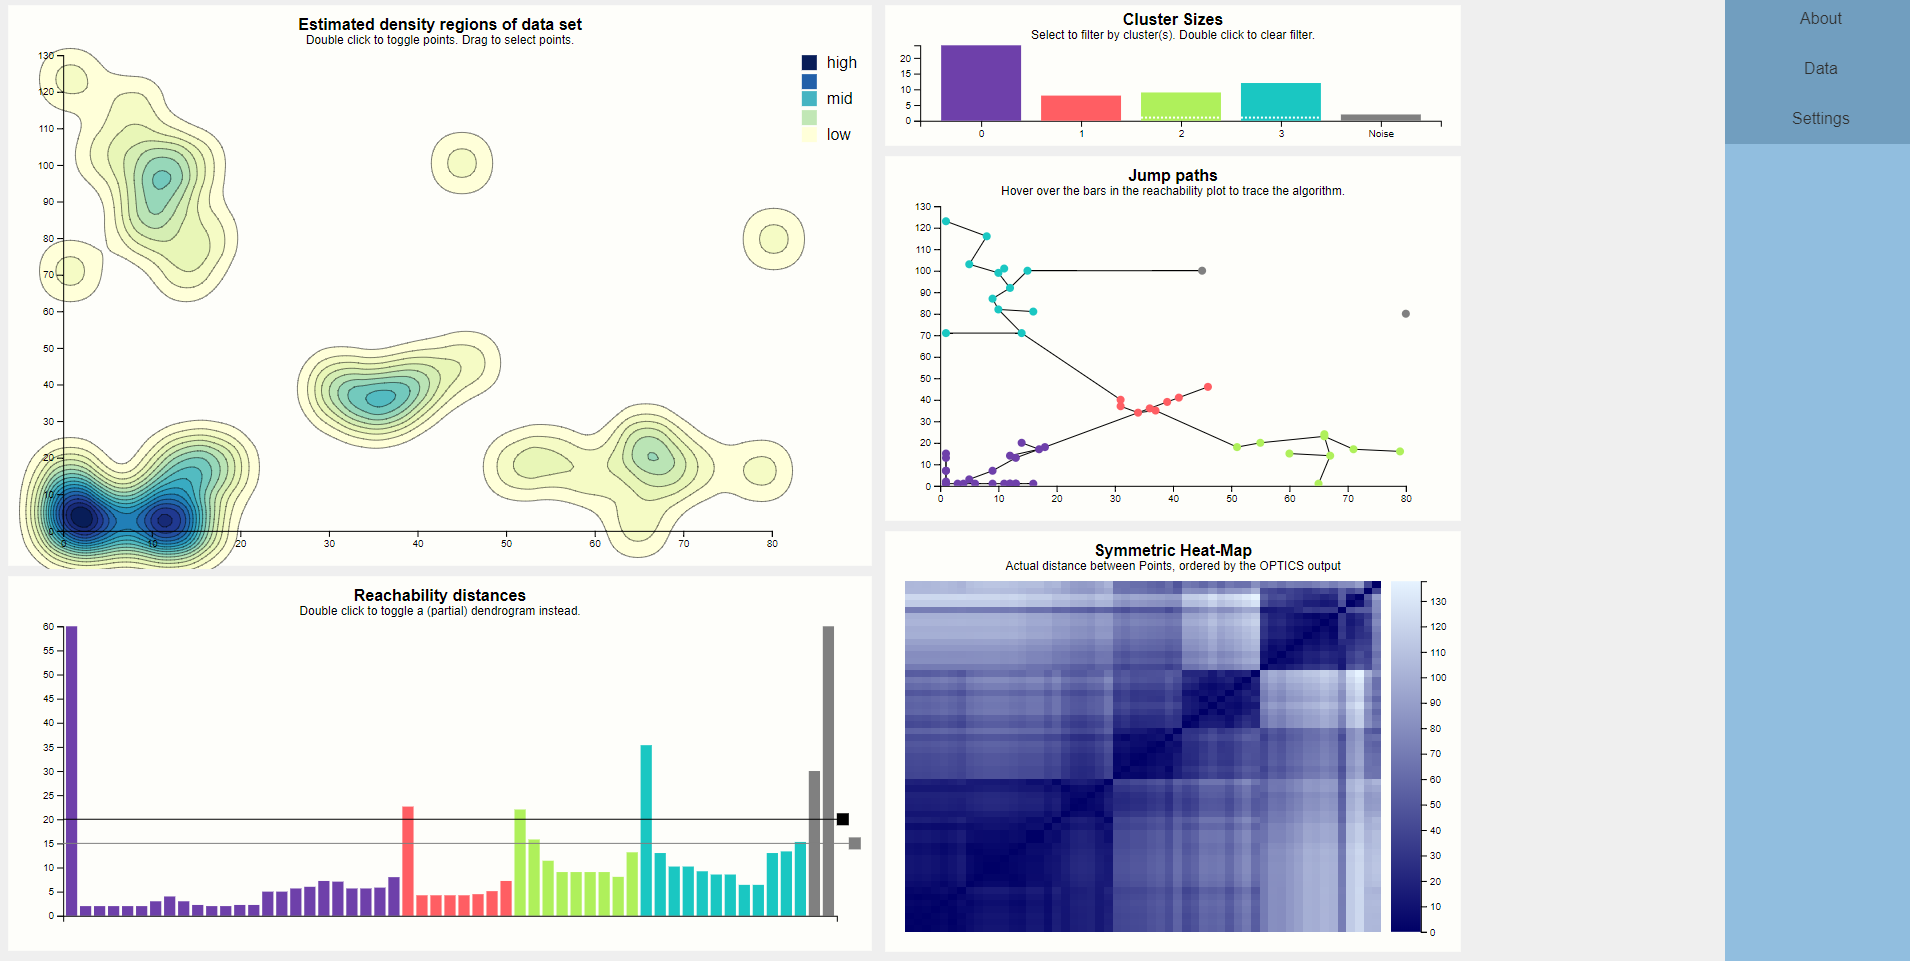
\includegraphics[width=0.5\textwidth]{/pictures/Scenario/1.PNG}

The logical next step is now to talk about the estimated density regions of the dataset where it is somewhat visualy obvious where the clusters are. An interesting question for the students would now be if they think, the left- or rightmost point in the bottom right cluster should still be part of the cluster.

\noindent
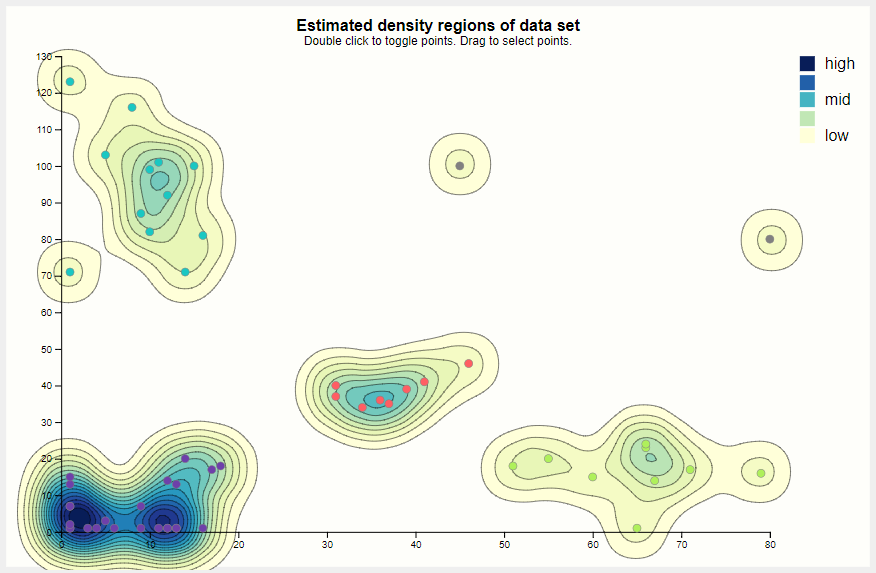
\includegraphics[width=0.5\textwidth]{/pictures/Scenario/2.PNG}

Moving the cutoff bar in the reachability plot around reveals, that the left point is removed first when moving the cutoff bar down.

\noindent
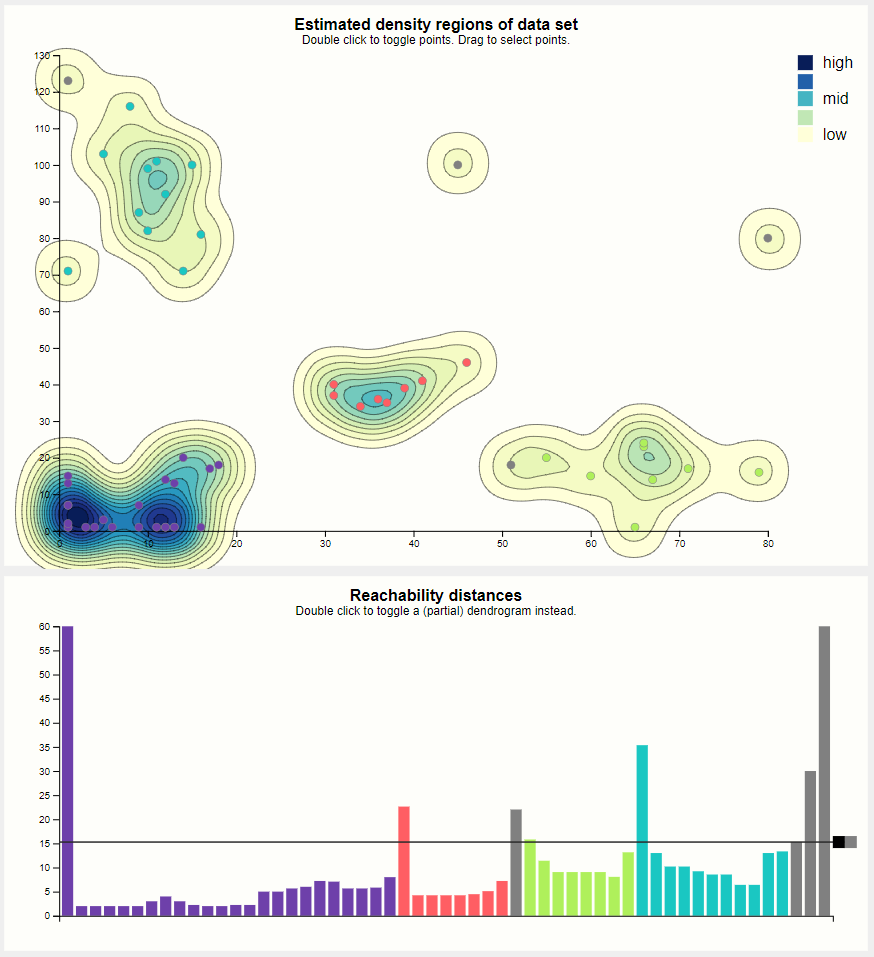
\includegraphics[width=0.5\textwidth]{/pictures/Scenario/3.PNG}

This can now be explained by mousing over the bars of the reachability plot and discussing how the reachability distance relates to the output of OPTICS, which is usualy just this reachability data.

While moving the cutoff bar arround it might also be interesting to see how it affects clusterpoints changing into noise and splitting clusters into smaller ones. A general overview might be had when looking at the cluster sizes plot.

\noindent
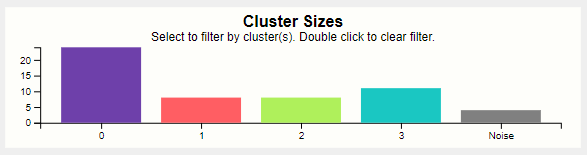
\includegraphics[width=0.5\textwidth]{/pictures/Scenario/4.PNG}

Whenever needed the teacher may also want to use the filtering in this plot to focus an a cluster or highlight something using the lasso in the density plot or the brush in the heatmap.

Explaining the algorithm step by step is supported by the jump paths plot where the teacher can follow each jump, by mousing over the corresponding bar in the reachability plot and zooming in the jump paths plot. An important point to make here is that the reachability value in the corresponding chart is not nesseserily equal to the actual distance between the two connected points. It is important to emphasise the influence of the  \emph{minPts} paramater on this value.

\noindent
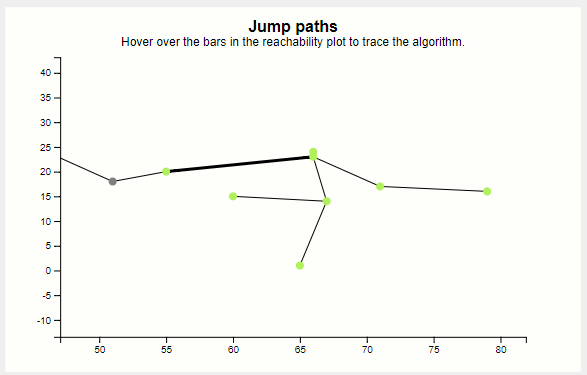
\includegraphics[width=0.5\textwidth]{/pictures/Scenario/5.PNG}

Next a general discussion may be had about what a good clustering actualy is. For this it may be a good idea to argue with our heat map.

\noindent
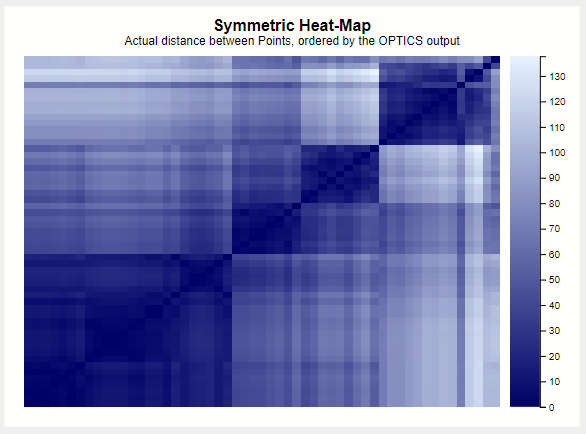
\includegraphics[width=0.5\textwidth]{/pictures/Scenario/6.PNG}

A good clustering will usualy produce a nice heatmap because points close to eachother in the data space will also be close to eachother in this plot and produce a rectangle or other recognizable shapes. Here the teacher can nicely show how a bad parameter set ( \emph{minPts}=8,  $\varepsilon$ =10) may produce a bad result.

\noindent
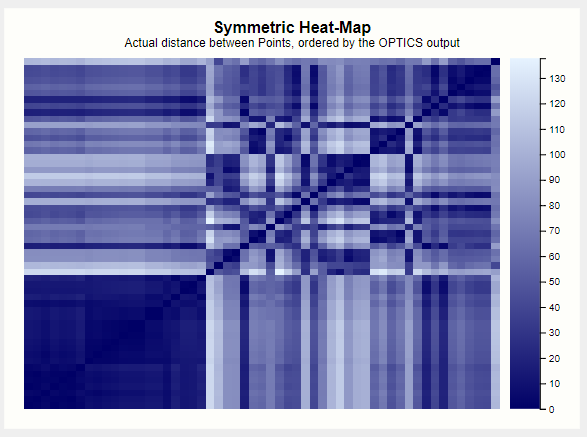
\includegraphics[width=0.5\textwidth]{/pictures/Scenario/7.PNG}

With those parameters no cutoff will produce a satisfactory clustering, unless this result was what we wanted. Here the teacher can explain, that we may actually still want a result like this, if there is reasoning behind the parameters, like explicitly not wanting clusters with less then 8 points reachable within the distance 10. This might throw out unwanted minor clusters and break weak links between clusters. Here would also be a good moment to talk about how reducing  $\varepsilon$ may improve the runtime of the algorithm greatly.

\noindent
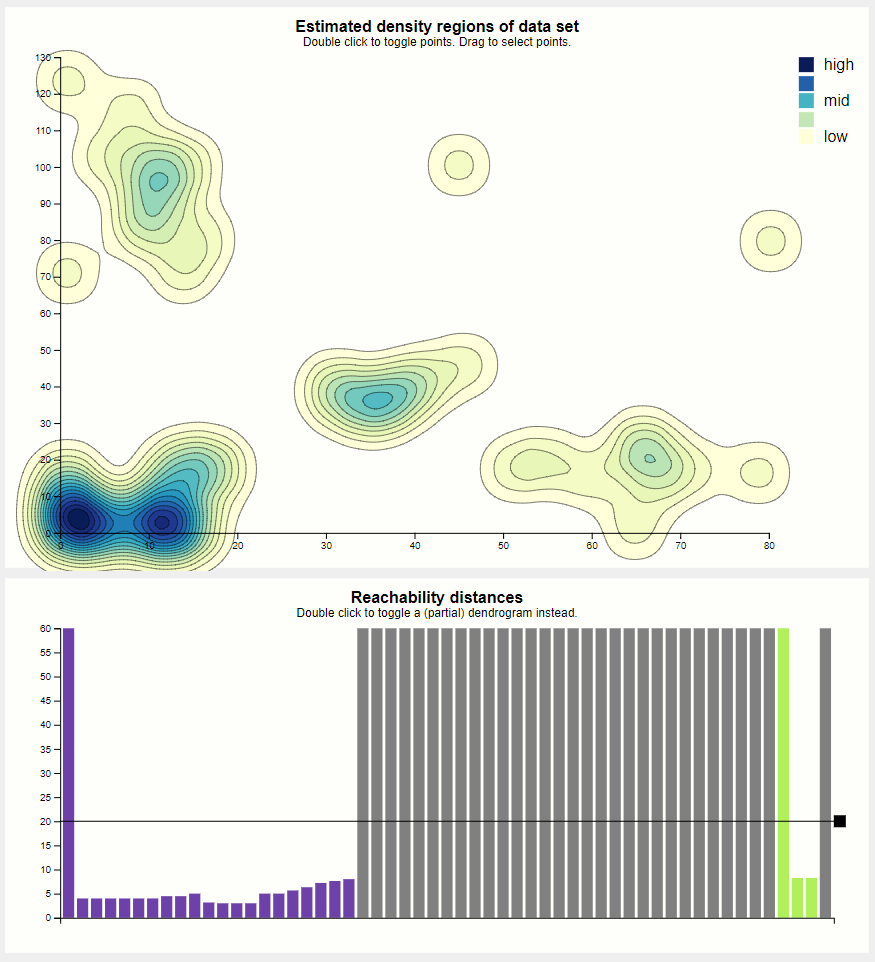
\includegraphics[width=0.5\textwidth]{/pictures/Scenario/8.PNG}

When the parameters were chosen well and the teacher wants to show and explore different clusterings, our dendogram can be shown.

\noindent
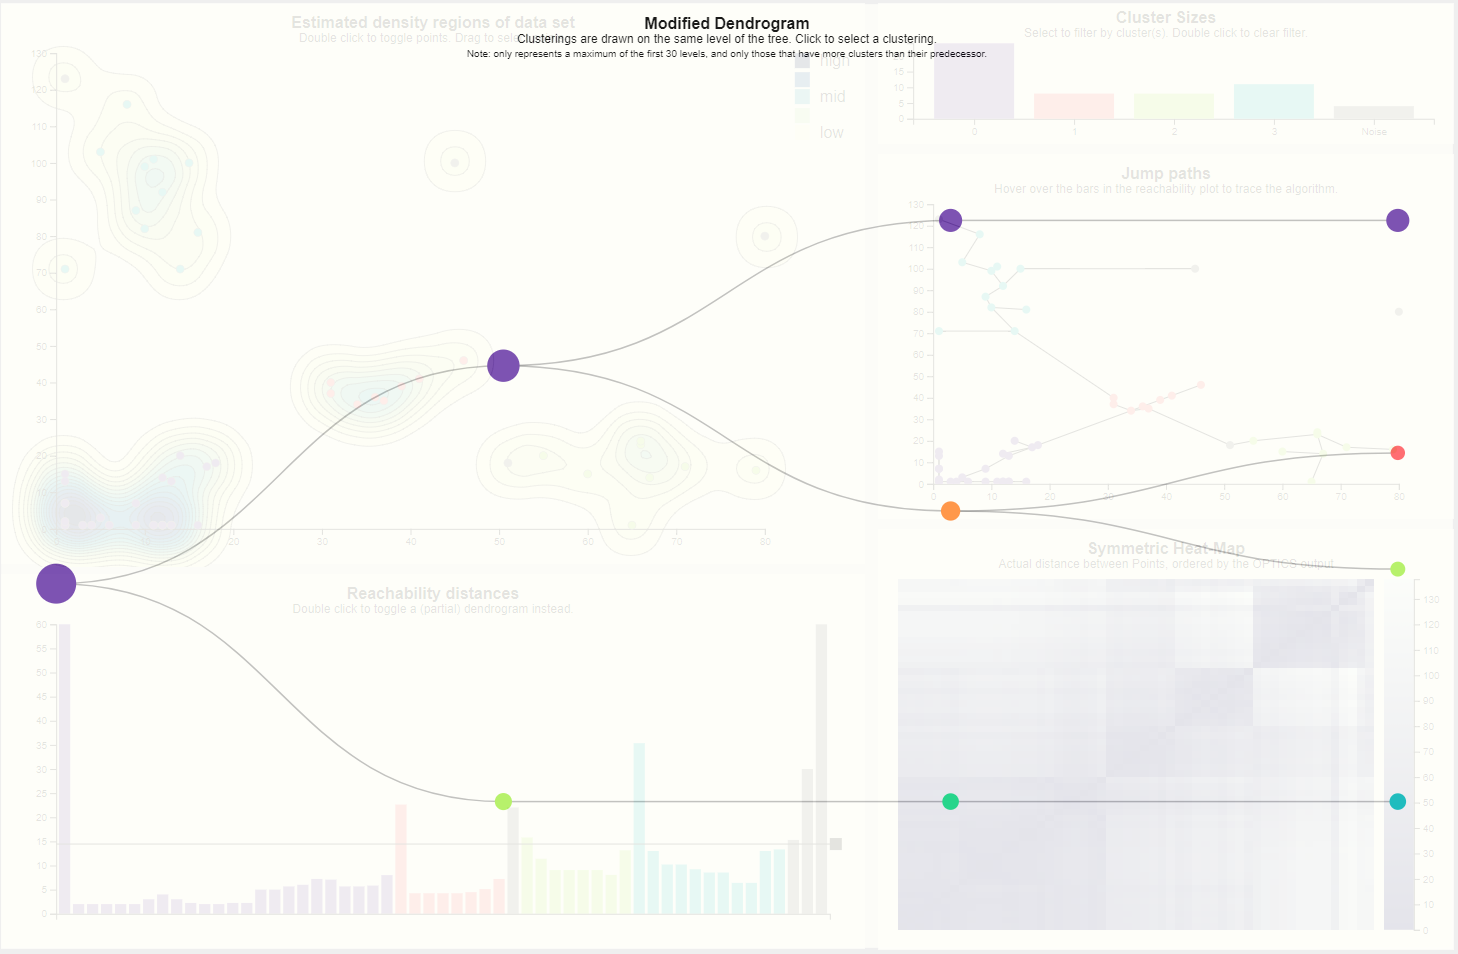
\includegraphics[width=0.5\textwidth]{/pictures/Scenario/9.PNG}

Clicking onto a column and leaving this view allows for quickly changing the cutoff to usefull settings. The cutoff can the be adjusted a little bit to achieve the right filtering of noise points in the data.

\subsection{Performance of the system}
\subsubsection{Computational Performance}

Computationally our tool is currently not well optimized. Since we implemented OPTICS ourselves we took a trivial approach and the runtime complexity for bad input parameters may reach $ O(n^{2}) $. For a more sophisticated implementation a server backend would be usefull as well as better optimized code.

A drawback of this is, that with current hardware working with a dataset larger than 400 points will result in stutter when interacting with different aspects of our tool.

\subsubsection{Visual Performance}
 Problems with huge datasets:
\begin{itemize}
\item The points in the plots may overlap a lot. It is possible to work around this by zooming in the jump paths plot and looking at parts of the data at a time.
\item The reachability plot may not be very nice anymore since the bars would be to thin to propperly distinguish.
\end{itemize}
Well working, even with huge datasets:
\begin{itemize}
\item The density plot should still give a good overview of the data, since it abstracts from single points.
\item The clustersizes plot should look the same, as long as there is not also a huge amount of clusters.
\item The heat map should always look good because it gives a hirachical overview and is zoomable. Shapes should still be recognizable.
\end{itemize}
\subsection{Evaluation/Feedback}
The Feedback we got consists of the course feedback given by our teachers and students durring our presentation of our prototype as well as from other users we questioned about our reworked prototype.
\subsubsection{Course Feedback}

First Feedback:

The first feedback we got was considered and implemented into our tool.

\noindent Seccond Feedback:

We were told, that our heat map shows ugly lines between the actual squares. This was due to rendering aritfacts from the browser and was easily fixed by changing a shape rendering propperty.

Another complaint was about the highlighting in the density plot. We have improved the highlighting behaviour and don't think this is a problem any more. We may be missunderstanding this feedback though, it is possible that what was actualy meant was that the highlighting does not work when the points are not visible. We want to keep this behaviour, because the user would otherwise have no idea where his highlighting comes from or be generaly confusing.

The last point made was questioning if our implementation visually scales well with large/realistic data sets. We think that it would, up to the point where the reachability distances plot can not be propperly read anymore because the bars get to thin. Another problem could be that the cluster sizes plot may get cramped when there are too many clusters. We targeted our implementation to the educational aspect and feel, that those problems are negligable because if someone wants to cluster a big data set they would want to use an optimized implementation anyway.

\subsubsection{User Feedback}
We were told, that the seccond cutoff line is not very nice or intuitive, so we removed it and replaced it with the new dendogram.

\section{Discussion}

\subsection{Strengths and weaknesses}
Strengths of our Tool:
\begin{itemize}
\item Allows to quickly explore clusterhirachies in small datasets.
\item Helps with learning and teaching about the OPTICS algorithm and density based clustering in general.
\item Helps understanding if the algorithm is fit for the problem the user aims to solve.
\item Default data sets give a nice overview over the capabilities of OPTICS for other data sets.
\item Shows additional meta imformation that may give additional insights. (dendogram/heat map)
\end{itemize}
Weaknesses of our Tool:
\begin{itemize}
\item It may be difficult to understand how OPTICS works without any knowledge about density based clustering or supervision.
\item May be to slow when working with larger datasets
\item May not be showing enought information when working with multidimensional data.
\end{itemize}
\subsection{Lessons we learned}

Durring this project we learned different new things.

\begin{itemize}
\item On top of what we learned about the d3 library in the visualization class, working with it on a custom project where we had to realize our own ideas made us dive deeper into its uses. This taught us how to work with it, what it is capable of as well as what it is not capable of and how to overcome those instances.
\item We learned a lot about creating nice visualizations, not only through the feedback we got, but usually from ourselves, when we did not like how something looked. Reworking what we did not like then showed us how not to visualize some things, which we will be able to apply in later projects.
\item We also learned about teamwork, especially because our team coordinated very well. We worked with the versioning tool git and besides sometimes needlessly having to merge code snippets, we think our task separation and joining of code parts worked flawlessly.
\end{itemize}

\section{Separation of Tasks}
\begin{table}[htb]
\centering
\caption{Milestone 1}
\label{my-label}
\begin{tabular}{@{} p{4cm}p{1cm}p{1cm} @{}}
\textbf{Task} & \textbf{Sonja} & \textbf{Christian} \\
 Website (Content) & 85\% & 15\%\\
 Idea & 15\% & 85\%\\
 Solution Sketch & 50\% & 50\%        
\end{tabular}
\end{table}
\FloatBarrier
\begin{table}[htb]
\centering
\caption{Milestone 2}
\label{my-label}
\begin{tabular}{@{} p{4cm}p{1cm}p{1cm} @{}}
\textbf{Task} & \textbf{Sonja} & \textbf{Christian} \\
 Chart explanation & 90\% & 10\%\\
 Mockup 1 & 0\% & 100\%\\
 Mockup 2 & 0\% & 100\%\\
 Mockup 3 & 100\% & 0\%\\
 Visualization Techniques & 100\% & 0\%\\
 Conclusion/Scenario of use & 0\% & 100\%\\
 Milestones & 70\% & 30\%        
\end{tabular}
\end{table}
\FloatBarrier
\begin{table}[htb]
\centering
\caption{Milestone 3}
\label{my-label}
\begin{tabular}{@{} p{4cm}p{1cm}p{1cm} @{}}
\textbf{Task} & \textbf{Sonja} & \textbf{Christian} \\
 Skeleton with Settings & 90\% & 10\%\\
 Charts (non interactive) & 40\% &  60\%\\
 Filter-Interaction & 50\% & 50\%\\
 Zoom/Pan-Interaction & 50\% & 50\%\\
 Highlight-Interaction & 60\% & 40\%\\
 Algorithm & 10\% & 90\%\\
 Web summary & 50\% & 50\%        
\end{tabular}
\end{table}
\FloatBarrier
\begin{table}[htb]
\centering
\caption{Milestone 4}
\label{my-label}
\begin{tabular}{@{} p{4cm}p{1cm}p{1cm} @{}}
\textbf{Task} & \textbf{Sonja} & \textbf{Christian} \\
 Dendogram & 100\% & 0\%\\
 Bugfixes & 40\% &  60\%\\
 Additional Data-Sets & 50\% & 50\%\\
 Paper & 50\% & 50\%
\end{tabular}
\end{table}
\FloatBarrier

\section{Conclusion}

Lorem ipsum dolor sit amet, consetetur sadipscing elitr, sed diam
nonumy eirmod tempor invidunt ut labore et dolore magna aliquyam erat,
sed diam voluptua. At vero eos et accusam et justo duo dolores et ea
rebum. Stet clita kasd gubergren, no sea takimata sanctus est Lorem
ipsum dolor sit amet. Lorem ipsum dolor sit amet, consetetur
sadipscing elitr, sed diam nonumy eirmod tempor invidunt ut labore et
dolore magna aliquyam erat, sed diam voluptua. At vero eos et accusam
et justo duo dolores et ea rebum. Stet clita kasd gubergren, no sea
takimata sanctus est Lorem ipsum dolor sit amet. Lorem ipsum dolor sit
amet, consetetur sadipscing elitr, sed diam nonumy eirmod tempor
invidunt ut labore et dolore magna aliquyam erat, sed diam
voluptua. At vero eos et accusam et justo duo dolores et ea
rebum.

%\bibliographystyle{abbrv}
\bibliographystyle{abbrv-doi}
%\bibliographystyle{abbrv-doi-narrow}
%\bibliographystyle{abbrv-doi-hyperref}
%\bibliographystyle{abbrv-doi-hyperref-narrow}

\bibliography{template}
\end{document}
